\documentclass[12pt]{article}   

% type user-defined commands here
\usepackage{geometry} % Required for adjusting page dimensions
\usepackage{placeins}
\usepackage{pifont}
\usepackage{hyperref}
\usepackage{amsmath,amsfonts,amsthm} % Math packages for equations
\usepackage{amssymb}
\usepackage[svgnames]{xcolor} % Enabling colors by their 'svgnames'
\usepackage{graphicx,caption,subcaption} % Required for adding images
\usepackage{insdljs,lcg,rangen} % random number generation
\usepackage{framed,adjustbox}
\usepackage[most]{tcolorbox} % colored comment box
\usepackage{booktabs}
\usepackage{cite,natbib}
\usepackage{tabu,multirow}
\usepackage{boldline,blindtext}
\usepackage[super]{nth} % typing nth in a nice format
\usepackage[official]{eurosym} % Euro symbol
\usepackage{fontawesome} % some cool symbols like hint

% page settings
\geometry{
top=1.5cm, % Top margin
bottom=1.5cm, % Bottom margin
left=2.5cm, % Left margin
right=2.5cm, % Right margin
includehead, % Include space for a header
includefoot, % Include space for a footer
%showframe, % Uncomment to show how the type block is set on the page
}

% generate random second color
\RandomZ{\R}{0}{255}%\R
\RandomZ{\G}{0}{255}%\G
\RandomZ{\B}{0}{255}%\B
\definecolor{ColorDef}{RGB}{\R,\G,\B}

\bibliographystyle{plain}
\newtheorem{thm}{Theorem}
\newtheorem{lem}[thm]{Lemma}
\newtheorem{prop}[thm]{Proposition}
\newtheorem{cor}{Corollary}
\newtheorem{conj}{Conjecture}
\theoremstyle{definition}
\newtheorem{defn}{Definition}
\newtheorem{exmp}{Example}
\newtheorem{rem}{Remark} 
\renewcommand{\qedsymbol}{\ensuremath{\blacksquare}}


\begin{document}

\title{\textcolor{ColorDef}{\textbf{Activity Report}}}   % type title between braces
\author{Leila Gharavi}         % type author(s) between braces
\date{January 1 - January 7}   % type date between braces
\maketitle
\vspace{-0.5cm}
\textcolor{ColorDef}{\hrule}
\vspace{-0.5cm}
\section*{}
\textbf{General Focus:} Name your main focus points (\emph{eg. Model Approximation})
\vspace{0.75cm}
\textcolor{ColorDef}{\hrule height 0.5pt}
\vspace{0.25cm}


\section*{Performed Activities}
\begin{itemize}
	
	\item \textbf{Leave:} \emph{n} days
	
	\item \textbf{Course Attending:} 
	\begin{itemize}
		\item \emph{Course 1} [\emph{Institute 1}]
		\item \emph{Course 2} [\emph{Institute 2}]
	\end{itemize}

	\smallskip
	\begin{tcolorbox}[fonttitle=\sffamily\large,colback=ColorDef!10,colframe=ColorDef,title=Title of the box,fontupper=\sffamily,breakable]	
		You can also use this colored box with a (removable) title to add a comment or extra information.
	\end{tcolorbox} 
	
	\item \textbf{MSc Supervision:} \emph{2 active} 
	\begin{itemize}
		\item \emph{Student 1} with \emph{Supervisor 1} -- the \nth{5} month (related to \emph{Problem 1})
		\item \emph{Student 2} with \emph{Supervisor 2} -- had kick-off meeting (related to \emph{Problem 2})
	\end{itemize}
	
	\item \textbf{Research Problem 1:} (see \hyperref[tech1]{\textbf{Research Problem 1}})
	\begin{itemize}
		\item Activity 11 \emph{e.g. Fixed some mistakes} 
		\item Activity 12 \emph{e.g. Changed some formulation}
		\item Activity 13 \emph{e.g. Discussion with someone over something}
	\end{itemize}

	\item \textbf{Research Problem 2:} (see \hyperref[tech2]{\textbf{Research Problem 2}})
	\begin{itemize} 
		\item Activity 21 \emph{e.g. Compared data with some other data} 
		\item Activity 22 \emph{e.g. Checked \cite{CitationKey}}
	\end{itemize}

\end{itemize}

% the following is a line, remove it if it is not nice or convenient
\vspace{0.25cm}
\textcolor{ColorDef}{\hrule height 0.5pt}
\vspace{0.25cm}

\section*{Proposed Future Activities} 
\begin{itemize}
	
	\item \textbf{Course Attending:} 
	\begin{itemize}
		\item \emph{Course 1} [\emph{Institute 1}] -- until February \nth{10}
		\item \emph{Course 2} [\emph{Institute 2}] -- until March \nth{3}
	\end{itemize}
	
	\item \textbf{MSc Supervision}
	
	\item \textbf{Teaching Assistance:} 
	\begin{itemize}
		\item \emph{Course Name} -- starts on January \nth{9} 
	\end{itemize}
	
	\item \textbf{Research Problem 1:}
	\begin{itemize}
		\item Activity 14 \emph{e.g. Investigate something} 
		\item Activity 15 \emph{e.g. Finish some draft}
	\end{itemize}
	
	\item \textbf{Research Problem 2:} 
	\begin{itemize} 			
		\item Activity 23 \emph{e.g. Implement the work in \cite{CitationKey}}
		\item Activity 24 \emph{e.g. pray it works!} 
	\end{itemize}
	
\end{itemize}

% the following is a line, remove it if it is not nice or convenient
\vspace{0.25cm}
\textcolor{ColorDef}{\hrule height 0.5pt}
\vspace{0.25cm}

\section*{Technical Details}\label{tech}

\subsection*{Research Problem 1}\label{tech1}

Consider a given cool equation such as 
\begin{equation}
	\dot{x} = f (x,u)
	\label{eq:coolformula}
\end{equation}
where $x$ is something and $u$ is something else, \dots

\FloatBarrier % if you want to see all the figures before the next section starts

\subsection*{Research Problem 2}\label{tech2}

For the sake of beauty, we will also include a cool picture here in Fig.~\ref{fig:coolfig}. 

	\begin{figure}[htbp]
	\centering
	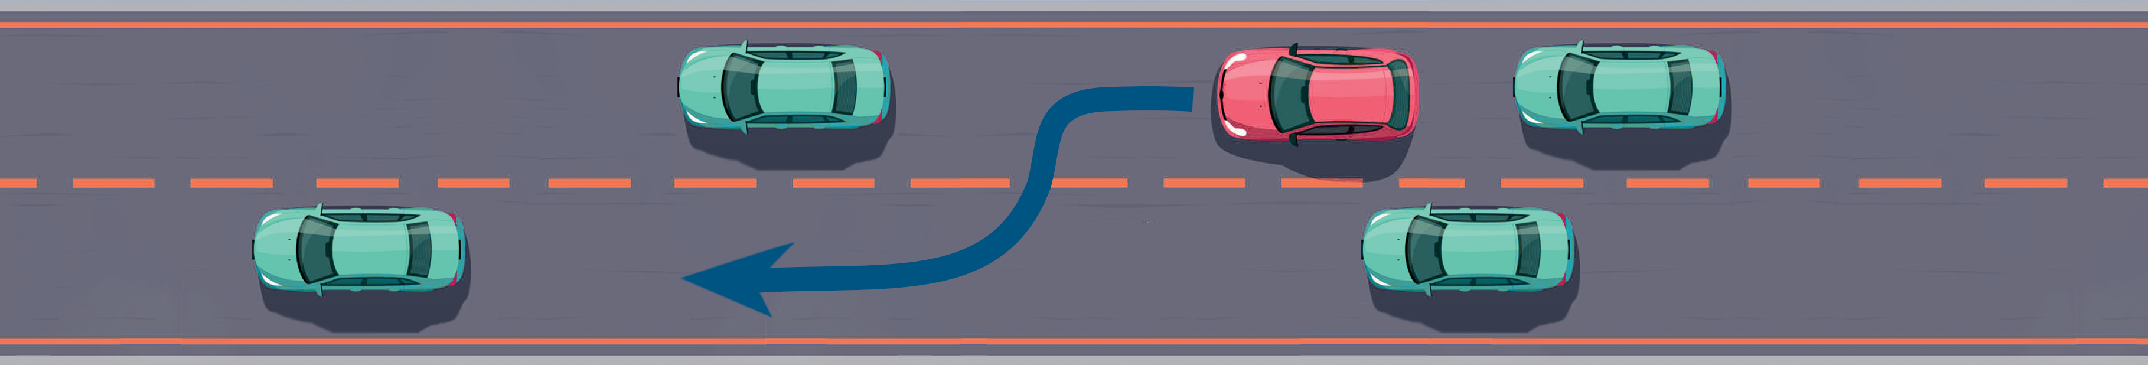
\includegraphics[width=0.7\textwidth]{Figures/Cars.pdf}
	\caption{Configuration of the single-track vehicle model}
	\label{fig:coolfig}
\end{figure}


\FloatBarrier % if you want to see all the figures before the next section starts

% the following is a line, remove it if it is not nice or convenient
\vspace{0.25cm}
\textcolor{ColorDef}{\hrule height 0.5pt}
\vspace{0.25cm}

\section*{Miscellaneous}

\begin{itemize}
\item \emph{Some [hopefully good] news}
\item \emph{Some topic for discussion}
\item \emph{Some question to ask}
\end{itemize}

% the following is a line, remove it if it is not nice or convenient
\vspace{0.25cm}
\textcolor{ColorDef}{\hrule height 0.5pt}
\vspace{0.25cm}

\bibliography{Citations}

\end{document}